%!TEX root = ../these.tex

\chapter{
  Описание формата файлов DBS
}
\label{app:dbs}

\newcommand{\dbsRecord}[1]{
  \noindent
  \begin{tabularx}{\textwidth}{|p{3em}|p{4em}|X|}
    \hline
    \multicolumn{1}{|c|}{Смещение} &
    \multicolumn{1}{c|}{Тип}      &
    \multicolumn{1}{c|}{Поле}     \\
    \hline
    #1
    \\
    \hline
  \end{tabularx}
}

\dbsRecord{
  4 & 5 & Превед Медвед!
}

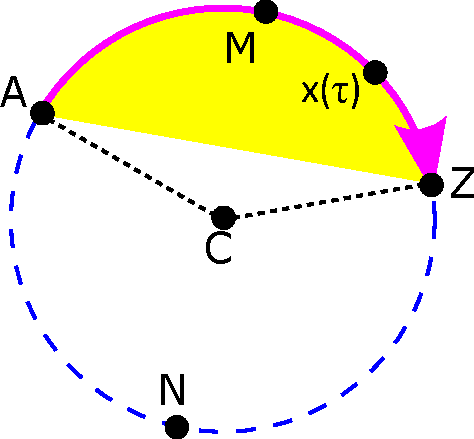
\includegraphics{arc.pdf}
